\section*{05/08/2022 --- Prova 1}
\markboth{Prova 1}{05/08/2022}
%	
	\textbf{\sffamily Questões}
	\begin{enumerate}
		\item [1)]
		Considerando os sistemas abaixo trace o retrato de fase dos mesmos e defina seus tipos.
		%
		\begin{itemize}
			\item [a)] 
			$\dis \frac{d^2 x}{dt^2} = 2x - \frac{dx}{dt} + u$
			{\hfill \tt (1.5)}
			
			\item [b)]			
			$\dis \frac{d^2 x}{dt^2} = -2x + \frac{dx}{dt} + u$
			{\hfill \tt (1.5)}
		\end{itemize}
		
		\item [2)]
		Considerando o sistema abaixo, determine o(s) ponto(s) de equilíbrio do mesmo e o(s) sistema(s) linearizado(s) tangente(s) associado(s).
		{\hfill \tt (3.0)}
		%
		\begin{align*}
			\frac{dx_1}{dt} &= -x_1(1-2x_2^2) - x_2 + ux_1 \\
			\frac{dx_2}{dt} &= x_1 - 1
		\end{align*}
		
		\item [3)]
		Determine uma função de Lyapunov e sua região de estabilidade do sistema abaixo. 
		{\hfill \tt (2.0)} \\
		Proponha um controle por Lyapunov para melhorar a performance do sistema 
		{\hfill \tt (2.0)}
		%
		\[
			\frac{d^2x}{dt^2} = -x - \frac{dx}{dt} + 
			                    \left(\frac{dx}{dt}\right)^3 + u + 1
		\]	
		%
	\end{enumerate}
	\rule{\textwidth}{0.5pt} \\
	\textbf{\sffamily Soluções}
	\begin{enumerate}
		\item [1)]
		Tomando a clássica escolha de estados $x_1=x$, $x_2=\dot{x}$, temos  para o sistema (a)
		%
		\[
			\dot{X} 
			= 
			AX + BU
			=
			\begin{pmatrix} 
				0 & 1 \\ 
				2 & -1 
			\end{pmatrix}
			X +
			\begin{pmatrix} 1 \\ 0 \end{pmatrix} u.
		\]
		%
		\textbf{Calculando os autovalores}
		\begin{align*}
			0 = \det(\lambda\I - A)         \iff 
			0 &= \lambda(\lambda+1) - 2  \\ \iff
			0 &= \lambda^2 + \lambda - 2 \\ \iff
			\lambda &= \lambda_1 = 1 \quad\vee\quad
			\lambda = \lambda_2 = -2.
		\end{align*}
		
		\textbf{Calculando os autovetores}
		\begin{align*}
			Av_1 &= \lambda_1 v_1 \iff 
			v_1 = x\begin{pmatrix} 1 & 1 \end{pmatrix}^T, 
			\quad\,\,\,\, x\in\R \\
			%
			Av_2 &= \lambda_1 v_2 \iff 
			v_2 = y\begin{pmatrix} 1 & -2 \end{pmatrix}^T, \quad y\in\R
		\end{align*}
	
		\textbf{Esboço do retrato de fase} \\
		Como $\lambda_2 < 0 < \lambda_1$, o RF será uma sela, e mais do que isso, os autovetores nos dizem que essa sela tem eixo instável na reta $x_2=x_1$ e estável na reta $x_2=-2x_1$.
		Segue o esboço.
		%
		\begin{figure}[H]\centering
			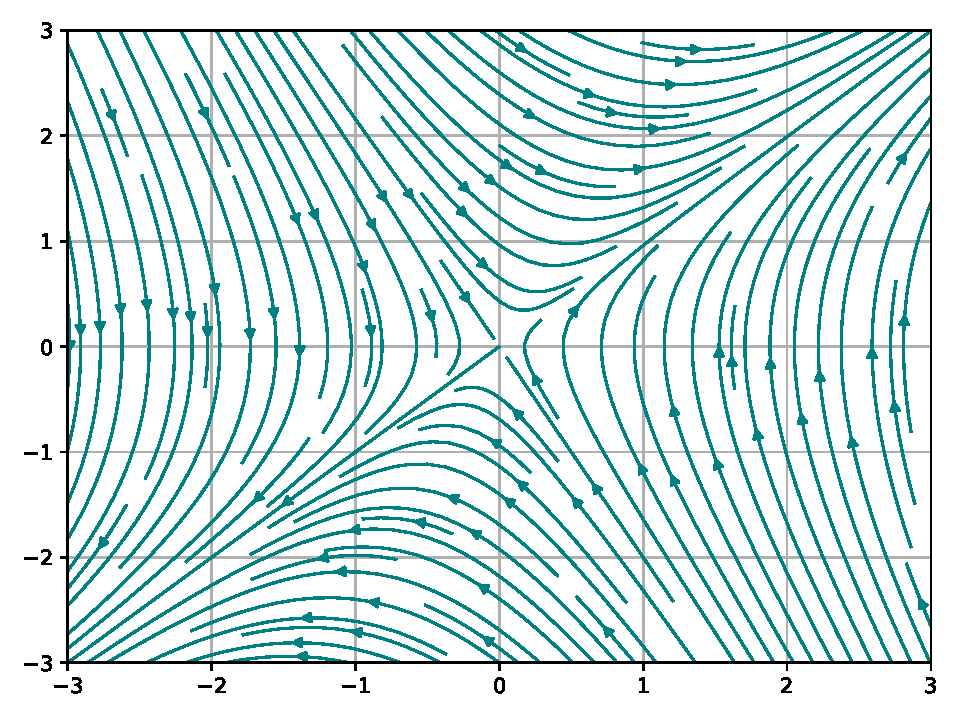
\includegraphics[width=7cm] {sela da prova1.pdf}
		\end{figure}
		%
		Para o sistema (b), 
		$A = 
		\begin{pmatrix} 
			0 & 1 \\
			-2 & 2
		\end{pmatrix}.$ \\
		
		\textbf{Calculando os autovalores}
		\begin{align*}
			0 = \det(\lambda\I - A)          \iff 
			0 &= \lambda(\lambda-2) + 2   \\ \iff
			0 &= \lambda^2 - 2\lambda + 2 \\ \iff
			\lambda &= \lambda_1 = 1+i \quad\vee\quad
			\lambda  = \lambda_2 = 1-i.
		\end{align*}
		%		
		\textbf{Esboço do retrato de fase} \\
		Como $\Re(\lambda_{1,2}) > 0$, o RF será um foco instável.
		Segue o esboço.
		%
		\begin{figure}[H]\centering
			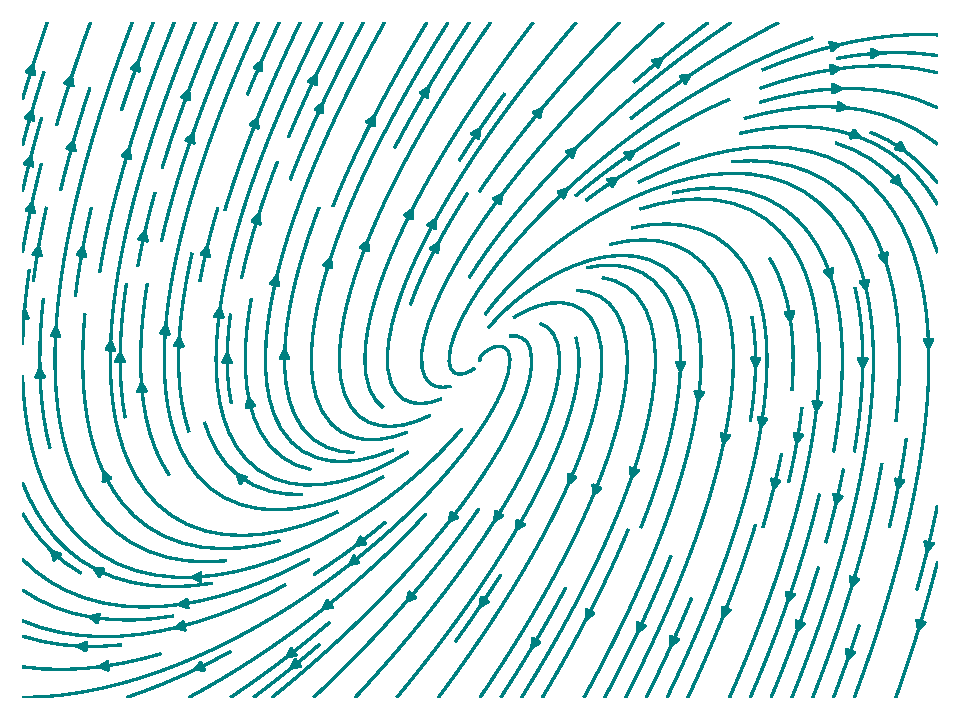
\includegraphics[width=7cm] {foco da prova1.pdf}
		\end{figure}
		%
		
		\item [2)]
		No ponto de equilíbrio $(\bar{x_1}, \bar{x_2})$, 
		$\dot{x}_1 = \dot{x}_2 = u = \bar{u} = 0$. 
		Substituindo nas EDOs, vem 
		%
		\begin{align*}
			\left\{	
				\begin{array}{l}
					0 = -\bar{x_1}(1 - 2\bar{x_2}^2) - \bar{x_2} \\
					0 = \bar{x_1} - 1
				\end{array}
			\right.
			\implies 
			\bar{x_1} = 1, \quad 2\bar{x_2}^2 - \bar{x_2} - 1.
		\end{align*}
		%
		Resolvendo a quadrática, chegamos a dois possíveis pontos de equilíbrio: 
		$P_1 = (1, 1)^T$ e $P_2 = (1, -1/2)^T$.
		Prosseguindo, linearizamos 
		$f_1(X;u) := \dot{x}_1$ e 
		$f_2(X;u) := \dot{x}_2$.
		Veja que
		%
		\[
			\begin{array}{lll}				
				\del_{x_1}f_1|_{(\bar{x_1}, \bar{x_2})}
				= 2\bar{x_2}^2-1  
				&
				\del_{x_2}f_1|_{(\bar{x_1}, \bar{x_2}) }
				= 4\bar{x_1x_2}-1
				&
				\del_u f_1|_{(\bar{x_1}, \bar{x_2})}
				= \bar{x_1} 
				\\
				\del_{x_1}f_2|_{(\bar{x_1}, \bar{x_2})}
				= 1 
				&
				\del_{x_2}f_2|_{(\bar{x_1}, \bar{x_2}) }
				= 0
				&
				\del_u f_2|_{(\bar{x_1}, \bar{x_2})}
				= 0 
			\end{array}
		\]
		%
		e portanto o linearizado em cada $P_j$ fica
		%
		\begin{align*}
			(\bar{x_1}, \bar{x_2}) = P_1 \implies
			\dot{X} &= 
			\begin{pmatrix} 
				1 & 3 \\ 1 & 0
			\end{pmatrix}
			(X-P_1) +
			\begin{pmatrix} 
				1 \\ 0
			\end{pmatrix}
			u,
			\\
			(\bar{x_1}, \bar{x_2}) = P_2 \implies
			\dot{X} &= 
			\begin{pmatrix} 
				-1/2 & -3 \\ 1 & 0
			\end{pmatrix}
			(X-P_2) +
			\begin{pmatrix} 
				1 \\ 0
			\end{pmatrix}
			u.
		\end{align*}
		
		\item [3)]
		Primeiro estabelecemos a estabilidade do sistema. Como este tem ponto de emquilíbrio $(x, \dot{x}) = (1, 0)$, tentamos $H$ de Lyapunov dada por 
		%
		\begin{equation}
			H(x(t)) = \frac{(x-1)^2}{2} + \frac{\dot{x}^2}{2}.
			\label{H da prova}
		\end{equation}
		%
		É fácil ver que $H$ acima é positiva para os pontos diferentes do equilíbrio e nula nele.
		O próximo passo é verificar a derivada de $H$ do tempo; temos
		%
		\begin{align*}
			\dot{H} &= \dot{x}(x-1) + \dot{x}\ddot{x} \\
			        &= \dot{x}(x-1+\ddot{x}) \\
			        &= \dot{x}(-\dot{x}+\dot{x}^3),
		\end{align*}
		%
		função nula no equilíbrio mas não necessariamente negativa fora dele. 
		Assim sendo, procuremos saber a região onde a estabilidade é garantida, isto é, $\dot{H}<0$ com $\dot{x}\neq 0$. 
		Vem
		%
		\begin{align*}
			\dot{x}(-\dot{x}+\dot{x}^3) < 0 \iff
			\dot{x}^2(\dot{x}^2-1) < 0      \iff
			\dot{x}^2-1 < 0                 \quad\therefore\quad
			0<|\dot{x}|<1.
		\end{align*}
		%
		A inequação acima define a região de estabilidade. 
		O retrato de fase do sistema mosrta que, realmente, esse intervalo abrange quase toda a região estável do sistema, embora não seja condição suficiente para a estabilidade.
		%
		\begin{figure}[H]\centering
			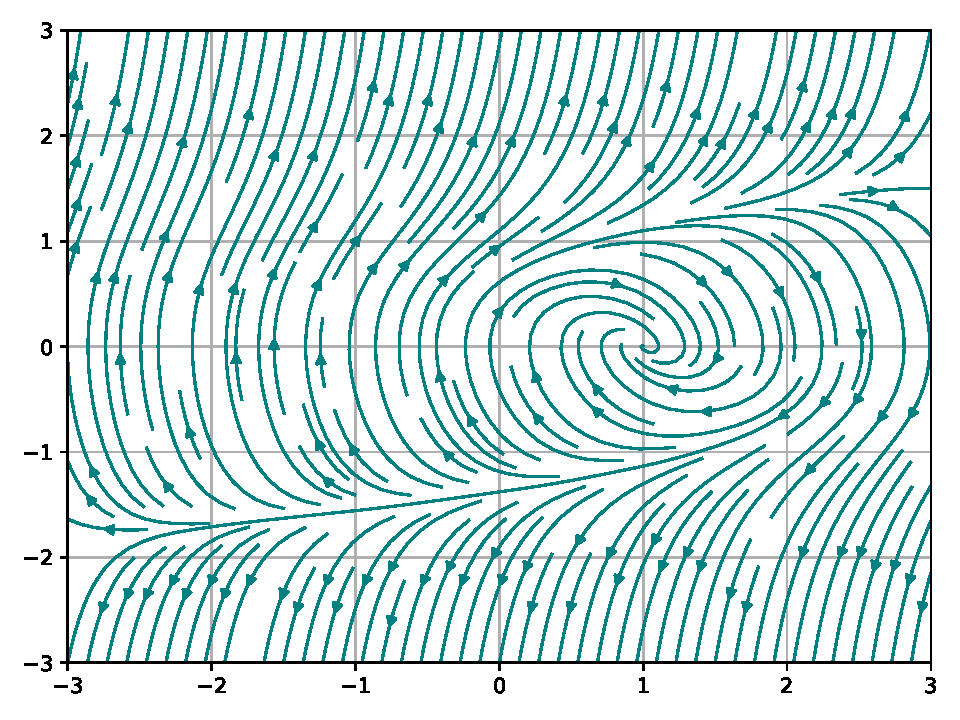
\includegraphics[width=7cm]{sistema de Lyapunov da prova1.pdf}
		\end{figure}
		%
		Agora, propomos controle de Lyapunov. Tomando a mesma $H$ de \eqref{H da prova}, a derivada se torna 
		%
		\begin{align*}
			\dot{H} &= \dot{x}(x - 1 + \ddot{x}) \\
			        &= \dot{x}(-\dot{x} + \dot{x}^3 + u),
		\end{align*}
		%
		e está claro que $u=-\dot{x}^3$, por exemplo, estabilizaria globalmente o sistema, melhorando sua performance.
	\end{enumerate}



















